%************************************************
\chapter{Experiment Data}
\label{chapter:experiment_data}
%************************************************

\section{Time and Space Complexities in Three Experiments}

This appendix chapter includes empirical data gathered using the
reflective tracing features of the underlying Funk garbage collected
memory system, upon which the virtual operating system is built.  This
low level memory tracing functionality allows easily tracing events at
any level of abstraction in the entire system using the Funk causal
reflective tracing features.  \autoref{table:experiment_data} shows a
list of figures showing data from three experiments.  In the first
experiment, the AI boots up and then perceives the world over time.
This experiment is a control that shows that the AI memory usage and
execution is stable if it does not have any goals and the physical
world is not changing.  In the second experiment, the reflective
learning is disabled.  In the third experiment, the AI reflectively
traces and builds models of the deliberative planning process.
Comparing the execution of the experiment with no reflective learning
with that of reflective learning shows a rough estimate of how much
more memory is used when the reflective learning about the
deliberative planning machine is enabled.  The evaluation chapter,
\autoref{chapter:evaluation}, has a more detailed analysis of the data
in this appendix, comparing the three experiments.

\begin{table}
  \centering
  \begin{tabular}{lllrr}
    ~         & \emph{Layer}      & \emph{Agency}      & \emph{Experiment Data}                                                      & \emph{Page} \\
    \hline AI &                   &                    & \autoref{figure:mind_plot-Gripper-1}                                        & \pageref{figure:mind_plot-Gripper-1} \\
    ~         & Reflective        &                    & \autoref{figure:mind_plot-Gripper-1-reflective}                             & \pageref{figure:mind_plot-Gripper-1-reflective} \\
    ~         &                   & Event Knowledge    & \autoref{figure:mind_plot-Gripper-1-reflective-reflective_event_knowledge}  & \pageref{figure:mind_plot-Gripper-1-reflective-reflective_event_knowledge} \\
    ~         &                   & Execution          & \autoref{figure:mind_plot-Gripper-1-reflective-execution}                   & \pageref{figure:mind_plot-Gripper-1-reflective-execution} \\
    ~         &                   & Imagination        & \autoref{figure:mind_plot-Gripper-1-reflective-imagination}                 & \pageref{figure:mind_plot-Gripper-1-reflective-imagination} \\
    ~         &                   & Object Type Goal   & \autoref{figure:mind_plot-Gripper-1-reflective-plan_object_type_goal}       & \pageref{figure:mind_plot-Gripper-1-reflective-plan_object_type_goal} \\
    ~         &                   & Plan               & \autoref{figure:mind_plot-Gripper-1-reflective-plan}                        & \pageref{figure:mind_plot-Gripper-1-reflective-plan} \\
    ~         &                   & Plan Bug Response  & \autoref{figure:mind_plot-Gripper-1-reflective-plan_bug_response}           & \pageref{figure:mind_plot-Gripper-1-reflective-plan_bug_response} \\
    ~         & Deliberative      &                    & \autoref{figure:mind_plot-Gripper-1-deliberative}                           & \pageref{figure:mind_plot-Gripper-1-deliberative} \\
    ~         &                   & Execution          & \autoref{figure:mind_plot-Gripper-1-deliberative-execution}                 & \pageref{figure:mind_plot-Gripper-1-deliberative-execution} \\
    ~         &                   & Imagination        & \autoref{figure:mind_plot-Gripper-1-deliberative-imagination}               & \pageref{figure:mind_plot-Gripper-1-deliberative-imagination} \\
    ~         &                   & Object Type Goal   & \autoref{figure:mind_plot-Gripper-1-deliberative-physical_object_type_goal} & \pageref{figure:mind_plot-Gripper-1-deliberative-physical_object_type_goal} \\
    ~         &                   & Plan               & \autoref{figure:mind_plot-Gripper-1-deliberative-plan}                      & \pageref{figure:mind_plot-Gripper-1-deliberative-plan} \\
    ~         & Learned Reactive  &                    & \autoref{figure:mind_plot-Gripper-1-learned_reactive}                       & \pageref{figure:mind_plot-Gripper-1-learned_reactive} \\
    ~         &                   & Physical Action    & \autoref{figure:mind_plot-Gripper-1-learned_reactive-physical}              & \pageref{figure:mind_plot-Gripper-1-learned_reactive-physical} \\
    ~         &                   & Physical Knowledge & \autoref{figure:mind_plot-Gripper-1-learned_reactive-physical_knowledge}    & \pageref{figure:mind_plot-Gripper-1-learned_reactive-physical_knowledge} \\
    ~         & Built-in Reactive &                    & \autoref{figure:mind_plot-Gripper-1-builtin_reactive}                       & \pageref{figure:mind_plot-Gripper-1-builtin_reactive} \\
    ~         &                   & Neural Plug        & \autoref{figure:mind_plot-Gripper-1-builtin_reactive-neural_plug}           & \pageref{figure:mind_plot-Gripper-1-builtin_reactive-neural_plug} \\
    ~         &                   & Physical Action    & \autoref{figure:mind_plot-Gripper-1-builtin_reactive-physical}              & \pageref{figure:mind_plot-Gripper-1-builtin_reactive-physical} \\
    ~         &                   & Sensory            & \autoref{figure:mind_plot-Gripper-1-builtin_reactive-sensory}               & \pageref{figure:mind_plot-Gripper-1-builtin_reactive-sensory} \\
  \end{tabular}
  \caption[Data from three experiments.]{Data from three experiments.}
  \label{table:experiment_data}
\end{table}

\newcommand{\experimentdatacommontablereference}{%
  {\mbox{\autoref{table:experiment_data}}} on
  {\mbox{page~\pageref{table:experiment_data}}} shows an index of
  the execution and memory usage from other causal scopes, such as
  the other layers or agencies of the AI, for these same three
  experiments.
}

\newcommand{\experimentdatacaptionbegin}[1]{
  \def\experimentdatacausegroupprettyname{#1}%
  All of the resources in the entire
  {\experimentdatacausegroupprettyname} have been causally traced and
  these two plots show: (top) the bytecode execution rate for the
  entire {\experimentdatacausegroupprettyname}, as well as (bottom)
  the memory footprint of the same causal scope.}

\newcommand{\experimentdatablocksworldexample}{
  \noindent\begin{minipage}{\textwidth/3}
    \centering%
    0 seconds\\
    \emph{Initialization}\\
    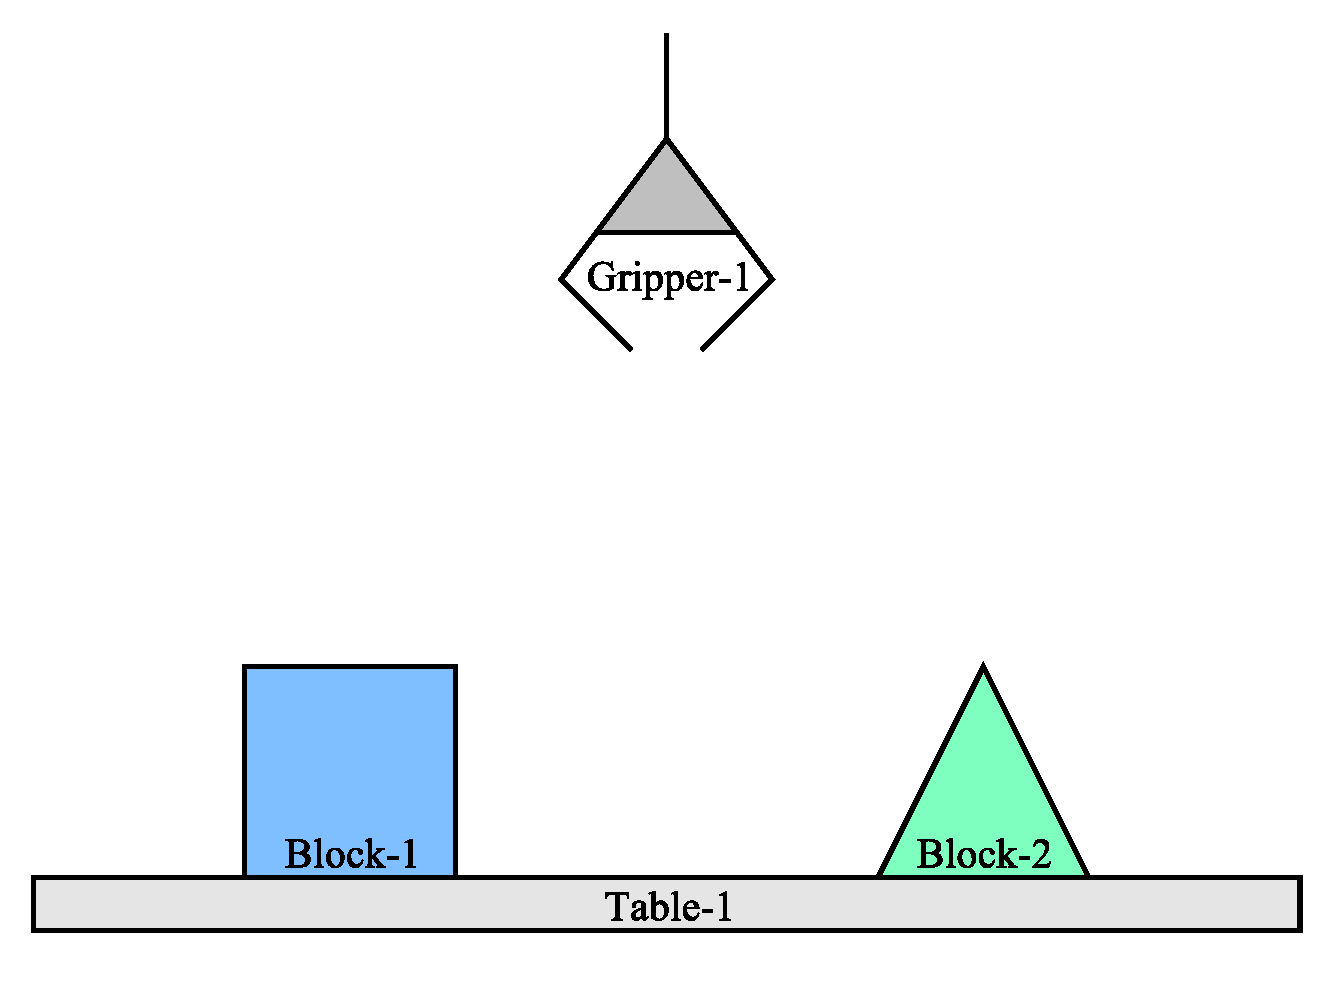
\includegraphics[width=3.5cm]{gfx/blocks_world_example-1}
  \end{minipage}%
    \noindent\begin{minipage}{\textwidth/3}
    \centering%
    15 seconds\\
    \emph{Deliberative Failure}\\
    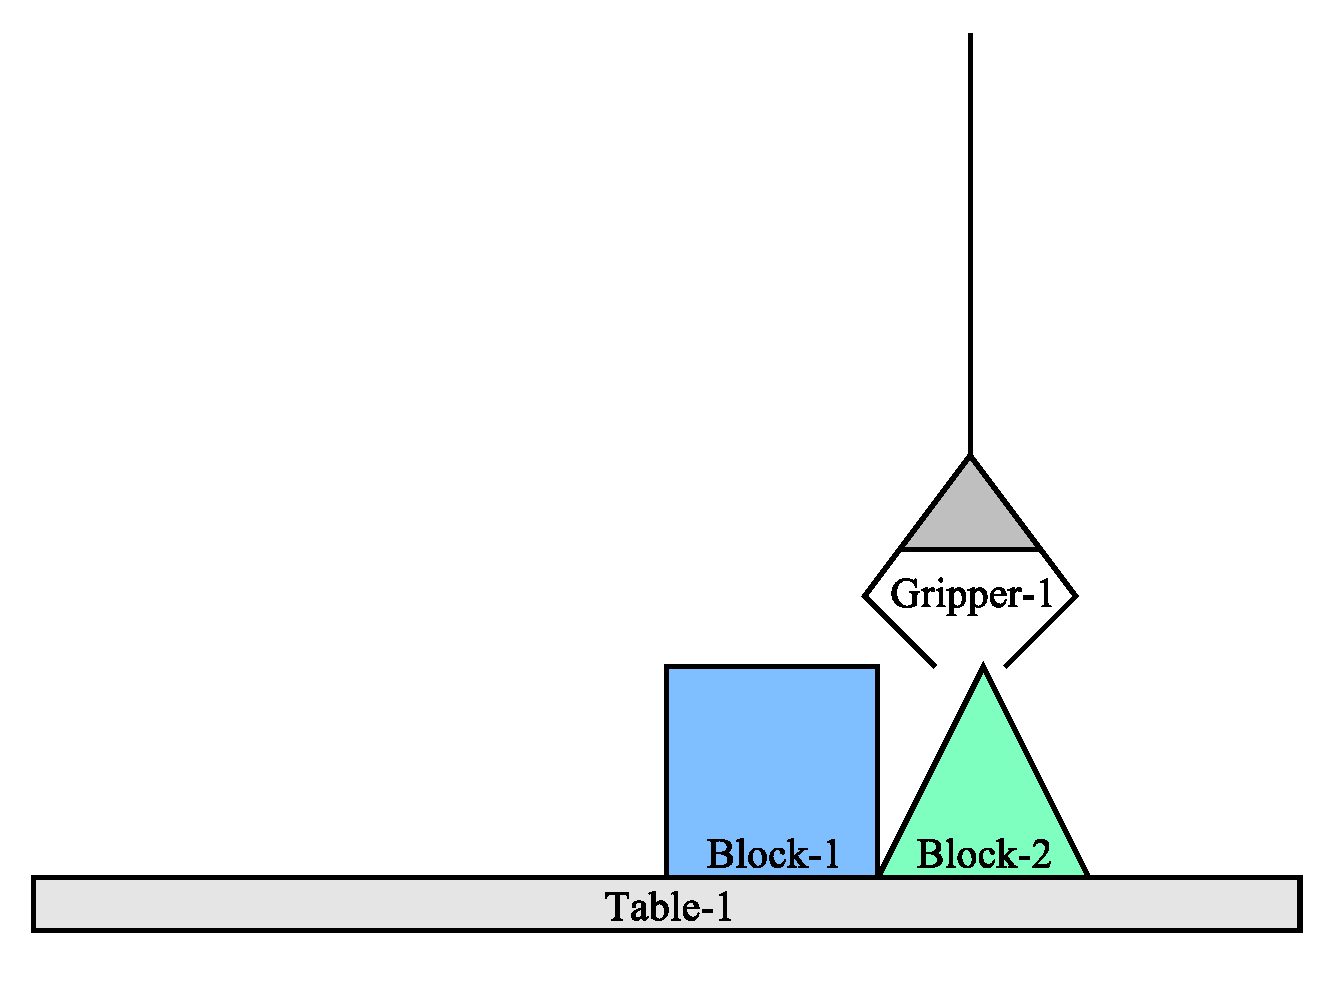
\includegraphics[width=3.5cm]{gfx/blocks_world_example-8}
  \end{minipage}%
  \noindent\begin{minipage}{\textwidth/3}
    \centering%
    25 seconds\\
    \emph{Reflective Success}\\
    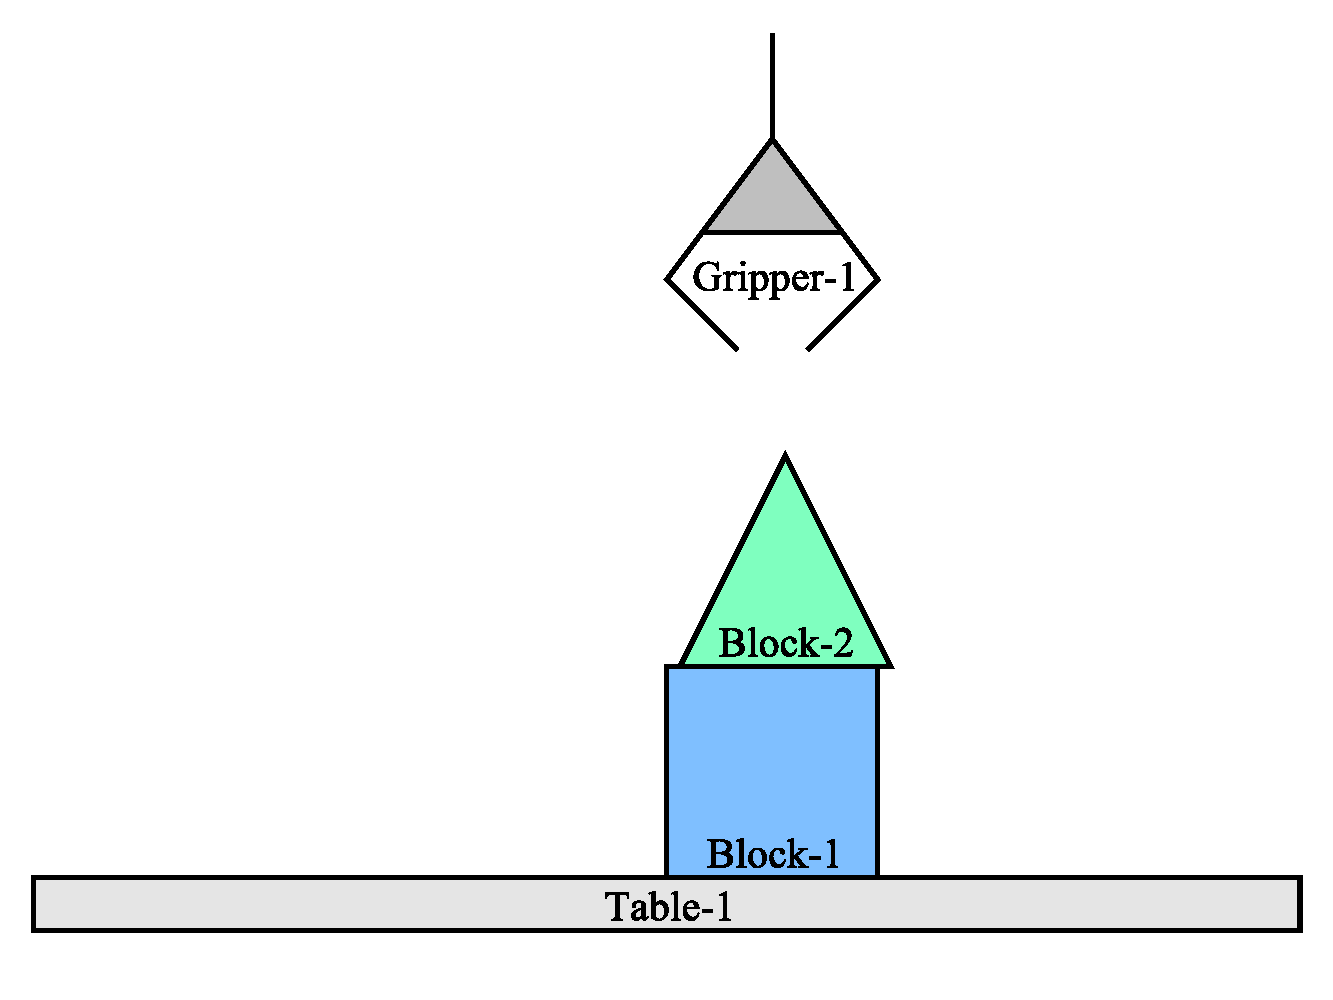
\includegraphics[width=3.5cm]{gfx/blocks_world_example-12}
  \end{minipage}%
}

% AI
{\newpage
  \noindent\begin{minipage}{\textwidth}
    \subsection{AI}
    \experimentcausegroupplots{\dataappendixmaxtime}
                              {\dataappendixexperimentonemaxtime}
                              {\dataappendixexperimenttwomaxtime}
                              {\dataappendixexperimentthreemaxtime}
                              {\dataappendixexperimentonename}
                              {\dataappendixexperimenttwoname}
                              {\dataappendixexperimentthreename}
                              {\dataappendixexperimentoneprettyname}
                              {\dataappendixexperimenttwoprettyname}
                              \experimentcausegroupplotscontinued{\dataappendixexperimentthreeprettyname}
                                                                 {mind_plot-Gripper-1}
                                                                 {AI}
                                                                 {\experimentdatacommontablereference}
                                                                 {4cm}
    \experimentdatablocksworldexample
    \captionof{figure}[Plots for the entire
      AI.]{\experimentdatacaptionbegin{AI}}
  \label{figure:mind_plot-Gripper-1}
  \end{minipage}
}
% reflective
{\newpage
  \noindent\begin{minipage}{\textwidth}
    \subsection{Reflective Layer}
    \experimentcausegroupplots{\dataappendixmaxtime}
                              {\dataappendixexperimentonemaxtime}
                              {\dataappendixexperimenttwomaxtime}
                              {\dataappendixexperimentthreemaxtime}
                              {\dataappendixexperimentonename}
                              {\dataappendixexperimenttwoname}
                              {\dataappendixexperimentthreename}
                              {\dataappendixexperimentoneprettyname}
                              {\dataappendixexperimenttwoprettyname}
                              \experimentcausegroupplotscontinued{\dataappendixexperimentthreeprettyname}
                                                                 {mind_plot-Gripper-1-reflective}
                                                                 {Reflective Layer}
                                                                 {\experimentdatacommontablereference}
                                                                 {4cm}
    \experimentdatablocksworldexample
    \captionof{figure}[Plots for the entire
      Reflective Layer.]{\experimentdatacaptionbegin{Reflective Layer}}
  \label{figure:mind_plot-Gripper-1-reflective}
  \end{minipage}
}
% reflective event knowledge
{\newpage
  \noindent\begin{minipage}{\textwidth}
    \subsubsection{Reflective Event Knowledge Agency}
    \experimentcausegroupplots{\dataappendixmaxtime}
                           {\dataappendixexperimentonemaxtime}
                           {\dataappendixexperimenttwomaxtime}
                           {\dataappendixexperimentthreemaxtime}
                           {\dataappendixexperimentonename}
                           {\dataappendixexperimenttwoname}
                           {\dataappendixexperimentthreename}
                           {\dataappendixexperimentoneprettyname}
                           {\dataappendixexperimenttwoprettyname}
                           \experimentcausegroupplotscontinued{\dataappendixexperimentthreeprettyname}
                                                              {mind_plot-Gripper-1-reflective-reflective_event_knowledge}
                                                              {Reflective Event Knowledge Agency}
                                                              {\experimentdatacommontablereference}
                                                              {4cm}
    \experimentdatablocksworldexample
    \captionof{figure}[Plots for the entire
      Reflective Event Knowledge Agency.]{\experimentdatacaptionbegin{Reflective Event Knowledge Agency}}
  \label{figure:mind_plot-Gripper-1-reflective-reflective_event_knowledge}
  \end{minipage}
}
% reflective execution
{\newpage
  \noindent\begin{minipage}{\textwidth}
    \subsubsection{Reflective Execution Agency}
    \experimentcausegroupplots{\dataappendixmaxtime}
                           {\dataappendixexperimentonemaxtime}
                           {\dataappendixexperimenttwomaxtime}
                           {\dataappendixexperimentthreemaxtime}
                           {\dataappendixexperimentonename}
                           {\dataappendixexperimenttwoname}
                           {\dataappendixexperimentthreename}
                           {\dataappendixexperimentoneprettyname}
                           {\dataappendixexperimenttwoprettyname}
                           \experimentcausegroupplotscontinued{\dataappendixexperimentthreeprettyname}
                                                              {mind_plot-Gripper-1-reflective-execution}
                                                              {Reflective Execution Agency}
                                                              {\experimentdatacommontablereference}
                                                              {4cm}
    \experimentdatablocksworldexample
    \captionof{figure}[Plots for the entire
      Reflective Execution Agency.]{\experimentdatacaptionbegin{Reflective Execution Agency}}
  \label{figure:mind_plot-Gripper-1-reflective-execution}
  \end{minipage}
}
% reflective imagination
{\newpage
  \noindent\begin{minipage}{\textwidth}
    \subsubsection{Reflective Imagination Agency}
    \experimentcausegroupplots{\dataappendixmaxtime}
                           {\dataappendixexperimentonemaxtime}
                           {\dataappendixexperimenttwomaxtime}
                           {\dataappendixexperimentthreemaxtime}
                           {\dataappendixexperimentonename}
                           {\dataappendixexperimenttwoname}
                           {\dataappendixexperimentthreename}
                           {\dataappendixexperimentoneprettyname}
                           {\dataappendixexperimenttwoprettyname}
                           \experimentcausegroupplotscontinued{\dataappendixexperimentthreeprettyname}
                                                              {mind_plot-Gripper-1-reflective-imagination}
                                                              {Reflective Imagination Agency}
                                                              {\experimentdatacommontablereference}
                                                              {4cm}
    \experimentdatablocksworldexample
    \captionof{figure}[Plots for the entire
      Reflective Imagination Agency.]{\experimentdatacaptionbegin{Reflective Imagination Agency}}
  \label{figure:mind_plot-Gripper-1-reflective-imagination}
  \end{minipage}
}
% reflective object type goal
{\newpage
  \noindent\begin{minipage}{\textwidth}
    \subsubsection{Reflective Object-Type-Goal Agency}
    \experimentcausegroupplots{\dataappendixmaxtime}
                           {\dataappendixexperimentonemaxtime}
                           {\dataappendixexperimenttwomaxtime}
                           {\dataappendixexperimentthreemaxtime}
                           {\dataappendixexperimentonename}
                           {\dataappendixexperimenttwoname}
                           {\dataappendixexperimentthreename}
                           {\dataappendixexperimentoneprettyname}
                           {\dataappendixexperimenttwoprettyname}
                           \experimentcausegroupplotscontinued{\dataappendixexperimentthreeprettyname}
                                                              {mind_plot-Gripper-1-reflective-plan_object_type_goal}
                                                              {Reflective Object-Type-Goal Agency}
                                                              {\experimentdatacommontablereference}
                                                              {4cm}
    \experimentdatablocksworldexample
    \captionof{figure}[Plots for the entire
      Reflective Object-Type-Goal Agency.]{\experimentdatacaptionbegin{Reflective Object-Type-Goal Agency}}
  \label{figure:mind_plot-Gripper-1-reflective-plan_object_type_goal}
  \end{minipage}
}
% reflective plan
{\newpage
  \noindent\begin{minipage}{\textwidth}
    \subsubsection{Reflective Plan Agency}
    \experimentcausegroupplots{\dataappendixmaxtime}
                           {\dataappendixexperimentonemaxtime}
                           {\dataappendixexperimenttwomaxtime}
                           {\dataappendixexperimentthreemaxtime}
                           {\dataappendixexperimentonename}
                           {\dataappendixexperimenttwoname}
                           {\dataappendixexperimentthreename}
                           {\dataappendixexperimentoneprettyname}
                           {\dataappendixexperimenttwoprettyname}
                           \experimentcausegroupplotscontinued{\dataappendixexperimentthreeprettyname}
                                                              {mind_plot-Gripper-1-reflective-plan}
                                                              {Reflective Plan Agency}
                                                              {\experimentdatacommontablereference}
                                                              {4.5cm}
    \experimentdatablocksworldexample
    \captionof{figure}[Plots for the entire
      Reflective Plan Agency.]{\experimentdatacaptionbegin{Reflective Plan Agency}}
  \label{figure:mind_plot-Gripper-1-reflective-plan}
  \end{minipage}
}
% reflective plan bug response
{\newpage
  \noindent\begin{minipage}{\textwidth}
    \subsubsection{Reflective Plan-Bug-Response Agency}
    \experimentcausegroupplots{\dataappendixmaxtime}
                           {\dataappendixexperimentonemaxtime}
                           {\dataappendixexperimenttwomaxtime}
                           {\dataappendixexperimentthreemaxtime}
                           {\dataappendixexperimentonename}
                           {\dataappendixexperimenttwoname}
                           {\dataappendixexperimentthreename}
                           {\dataappendixexperimentoneprettyname}
                           {\dataappendixexperimenttwoprettyname}
                           \experimentcausegroupplotscontinued{\dataappendixexperimentthreeprettyname}
                                                              {mind_plot-Gripper-1-reflective-plan_bug_response}
                                                              {Reflective Plan-Bug-Response Agency}
                                                              {\experimentdatacommontablereference}
                                                              {4.5cm}
    \experimentdatablocksworldexample
    \captionof{figure}[Plots for the entire
      Reflective Plan-Bug-Response Agency.]{\experimentdatacaptionbegin{Reflective Plan-Bug-Response Agency}}
  \label{figure:mind_plot-Gripper-1-reflective-plan_bug_response}
  \end{minipage}
}
% deliberative
{\newpage
  \noindent\begin{minipage}{\textwidth}
    \subsection{Deliberative Layer}
    \experimentcausegroupplots{\dataappendixmaxtime}
                           {\dataappendixexperimentonemaxtime}
                           {\dataappendixexperimenttwomaxtime}
                           {\dataappendixexperimentthreemaxtime}
                           {\dataappendixexperimentonename}
                           {\dataappendixexperimenttwoname}
                           {\dataappendixexperimentthreename}
                           {\dataappendixexperimentoneprettyname}
                           {\dataappendixexperimenttwoprettyname}
                           \experimentcausegroupplotscontinued{\dataappendixexperimentthreeprettyname}
                                                              {mind_plot-Gripper-1-deliberative}
                                                              {Deliberative Layer}
                                                              {\experimentdatacommontablereference}
                                                              {4cm}
    \experimentdatablocksworldexample
    \captionof{figure}[Plots for the entire
      Deliberative Layer.]{\experimentdatacaptionbegin{Deliberative Layer}}
  \label{figure:mind_plot-Gripper-1-deliberative}
  \end{minipage}
}
% deliberative execution
{\newpage
  \noindent\begin{minipage}{\textwidth}
    \subsubsection{Deliberative Execution Agency}
    \experimentcausegroupplots{\dataappendixmaxtime}
                           {\dataappendixexperimentonemaxtime}
                           {\dataappendixexperimenttwomaxtime}
                           {\dataappendixexperimentthreemaxtime}
                           {\dataappendixexperimentonename}
                           {\dataappendixexperimenttwoname}
                           {\dataappendixexperimentthreename}
                           {\dataappendixexperimentoneprettyname}
                           {\dataappendixexperimenttwoprettyname}
                           \experimentcausegroupplotscontinued{\dataappendixexperimentthreeprettyname}
                                                              {mind_plot-Gripper-1-deliberative-execution}
                                                              {Deliberative Execution Agency}
                                                              {\experimentdatacommontablereference}
                                                              {4cm}
    \experimentdatablocksworldexample
    \captionof{figure}[Plots for the entire
      Deliberative Execution Agency.]{\experimentdatacaptionbegin{Deliberative Execution Agency}}
  \label{figure:mind_plot-Gripper-1-deliberative-execution}
  \end{minipage}
}
% deliberative imagination
{\newpage
  \noindent\begin{minipage}{\textwidth}
    \subsubsection{Deliberative Imagination Agency}
    \experimentcausegroupplots{\dataappendixmaxtime}
                           {\dataappendixexperimentonemaxtime}
                           {\dataappendixexperimenttwomaxtime}
                           {\dataappendixexperimentthreemaxtime}
                           {\dataappendixexperimentonename}
                           {\dataappendixexperimenttwoname}
                           {\dataappendixexperimentthreename}
                           {\dataappendixexperimentoneprettyname}
                           {\dataappendixexperimenttwoprettyname}
                           \experimentcausegroupplotscontinued{\dataappendixexperimentthreeprettyname}
                                                              {mind_plot-Gripper-1-deliberative-imagination}
                                                              {Deliberative Imagination Agency}
                                                              {\experimentdatacommontablereference}
                                                              {4cm}
    \experimentdatablocksworldexample
    \captionof{figure}[Plots for the entire
      Deliberative Imagination Agency.]{\experimentdatacaptionbegin{Deliberative Imagination Agency}}
  \label{figure:mind_plot-Gripper-1-deliberative-imagination}
  \end{minipage}
}
% deliberative object type goal
{\newpage
  \noindent\begin{minipage}{\textwidth}
    \subsubsection{Deliberative Object Type Goal Agency}
    \experimentcausegroupplots{\dataappendixmaxtime}
                           {\dataappendixexperimentonemaxtime}
                           {\dataappendixexperimenttwomaxtime}
                           {\dataappendixexperimentthreemaxtime}
                           {\dataappendixexperimentonename}
                           {\dataappendixexperimenttwoname}
                           {\dataappendixexperimentthreename}
                           {\dataappendixexperimentoneprettyname}
                           {\dataappendixexperimenttwoprettyname}
                           \experimentcausegroupplotscontinued{\dataappendixexperimentthreeprettyname}
                                                              {mind_plot-Gripper-1-deliberative-physical_object_type_goal}
                                                              {Deliberative Object Type Goal Agency}
                                                              {\experimentdatacommontablereference}
                                                              {4cm}
    \experimentdatablocksworldexample
    \captionof{figure}[Plots for the entire
      Deliberative Object Type Goal Agency.]{\experimentdatacaptionbegin{Deliberative Object Type Goal Agency}}
  \label{figure:mind_plot-Gripper-1-deliberative-physical_object_type_goal}
  \end{minipage}
}
% deliberative plan
{\newpage
  \noindent\begin{minipage}{\textwidth}
    \subsubsection{Deliberative Plan Agency}
    \experimentcausegroupplots{\dataappendixmaxtime}
                           {\dataappendixexperimentonemaxtime}
                           {\dataappendixexperimenttwomaxtime}
                           {\dataappendixexperimentthreemaxtime}
                           {\dataappendixexperimentonename}
                           {\dataappendixexperimenttwoname}
                           {\dataappendixexperimentthreename}
                           {\dataappendixexperimentoneprettyname}
                           {\dataappendixexperimenttwoprettyname}
                           \experimentcausegroupplotscontinued{\dataappendixexperimentthreeprettyname}
                                                              {mind_plot-Gripper-1-deliberative-plan}
                                                              {Deliberative Plan Agency}
                                                              {\experimentdatacommontablereference}
                                                              {4cm}
    \experimentdatablocksworldexample
    \captionof{figure}[Plots for the entire
      Deliberative Plan Agency.]{\experimentdatacaptionbegin{Deliberative Plan Agency}}
  \label{figure:mind_plot-Gripper-1-deliberative-plan}
  \end{minipage}
}
% learned reactive
{\newpage
  \noindent\begin{minipage}{\textwidth}
    \subsection{Learned Reactive Layer}
    \experimentcausegroupplots{\dataappendixmaxtime}
                           {\dataappendixexperimentonemaxtime}
                           {\dataappendixexperimenttwomaxtime}
                           {\dataappendixexperimentthreemaxtime}
                           {\dataappendixexperimentonename}
                           {\dataappendixexperimenttwoname}
                           {\dataappendixexperimentthreename}
                           {\dataappendixexperimentoneprettyname}
                           {\dataappendixexperimenttwoprettyname}
                           \experimentcausegroupplotscontinued{\dataappendixexperimentthreeprettyname}
                                                              {mind_plot-Gripper-1-learned_reactive}
                                                              {Learned Reactive Layer}
                                                              {\experimentdatacommontablereference}
                                                              {4cm}
    \experimentdatablocksworldexample
    \captionof{figure}[Plots for the entire
      Learned Reactive Layer.]{\experimentdatacaptionbegin{Learned Reactive Layer}}
  \label{figure:mind_plot-Gripper-1-learned_reactive}
  \end{minipage}
}
% learned reactive physical action
{\newpage
  \noindent\begin{minipage}{\textwidth}
    \subsubsection{Learned Reactive Physical Action Agency}
    \experimentcausegroupplots{\dataappendixmaxtime}
                           {\dataappendixexperimentonemaxtime}
                           {\dataappendixexperimenttwomaxtime}
                           {\dataappendixexperimentthreemaxtime}
                           {\dataappendixexperimentonename}
                           {\dataappendixexperimenttwoname}
                           {\dataappendixexperimentthreename}
                           {\dataappendixexperimentoneprettyname}
                           {\dataappendixexperimenttwoprettyname}
                           \experimentcausegroupplotscontinued{\dataappendixexperimentthreeprettyname}
                                                              {mind_plot-Gripper-1-learned_reactive-physical}
                                                              {Learned Reactive Physical Action Agency}
                                                              {\experimentdatacommontablereference}
                                                              {4cm}
    \experimentdatablocksworldexample
    \captionof{figure}[Plots for the entire
      Learned Reactive Physical Action Agency.]{\experimentdatacaptionbegin{Learned Reactive Physical Action Agency}}
  \label{figure:mind_plot-Gripper-1-learned_reactive-physical}
  \end{minipage}
}
% learned reactive physical knowledge
{\newpage
  \noindent\begin{minipage}{\textwidth}
    \subsubsection{Learned Reactive Physical-Knowledge Agency}
    \experimentcausegroupplots{\dataappendixmaxtime}
                           {\dataappendixexperimentonemaxtime}
                           {\dataappendixexperimenttwomaxtime}
                           {\dataappendixexperimentthreemaxtime}
                           {\dataappendixexperimentonename}
                           {\dataappendixexperimenttwoname}
                           {\dataappendixexperimentthreename}
                           {\dataappendixexperimentoneprettyname}
                           {\dataappendixexperimenttwoprettyname}
                           \experimentcausegroupplotscontinued{\dataappendixexperimentthreeprettyname}
                                                              {mind_plot-Gripper-1-learned_reactive-physical_knowledge}
                                                              {Learned Reactive Physical-Knowledge Agency}
                                                              {\experimentdatacommontablereference}
                                                              {4cm}
    \experimentdatablocksworldexample
    \captionof{figure}[Plots for the entire
      Learned Reactive Physical-Knowledge Agency.]{\experimentdatacaptionbegin{Learned Reactive Physical-Knowledge Agency}}
  \label{figure:mind_plot-Gripper-1-learned_reactive-physical_knowledge}
  \end{minipage}
}
% built-in reactive
{\newpage
  \noindent\begin{minipage}{\textwidth}
    \subsection{Built-in Reactive Layer}
    \experimentcausegroupplots{\dataappendixmaxtime}
                           {\dataappendixexperimentonemaxtime}
                           {\dataappendixexperimenttwomaxtime}
                           {\dataappendixexperimentthreemaxtime}
                           {\dataappendixexperimentonename}
                           {\dataappendixexperimenttwoname}
                           {\dataappendixexperimentthreename}
                           {\dataappendixexperimentoneprettyname}
                           {\dataappendixexperimenttwoprettyname}
                           \experimentcausegroupplotscontinued{\dataappendixexperimentthreeprettyname}
                                                              {mind_plot-Gripper-1-builtin_reactive}
                                                              {Built-in Reactive Layer}
                                                              {\experimentdatacommontablereference}
                                                              {4cm}
    \experimentdatablocksworldexample
    \captionof{figure}[Plots for the entire
      Built-in Reactive Layer.]{\experimentdatacaptionbegin{Built-in Reactive Layer}}
  \label{figure:mind_plot-Gripper-1-builtin_reactive}
  \end{minipage}
}
% built-in reactive neural plug
{\newpage
  \noindent\begin{minipage}{\textwidth}
    \subsubsection{Built-in Reactive Neural Plug Agency}
    \experimentcausegroupplots{\dataappendixmaxtime}
                           {\dataappendixexperimentonemaxtime}
                           {\dataappendixexperimenttwomaxtime}
                           {\dataappendixexperimentthreemaxtime}
                           {\dataappendixexperimentonename}
                           {\dataappendixexperimenttwoname}
                           {\dataappendixexperimentthreename}
                           {\dataappendixexperimentoneprettyname}
                           {\dataappendixexperimenttwoprettyname}
                           \experimentcausegroupplotscontinued{\dataappendixexperimentthreeprettyname}
                                                              {mind_plot-Gripper-1-builtin_reactive-neural_plug}
                                                              {Built-in Reactive Neural Plug Agency}
                                                              {\experimentdatacommontablereference}
                                                              {4cm}
    \experimentdatablocksworldexample
    \captionof{figure}[Plots for the entire
      Built-in Reactive Neural Plug Agency.]{\experimentdatacaptionbegin{Built-in Reactive Neural Plug Agency}}
  \label{figure:mind_plot-Gripper-1-builtin_reactive-neural_plug}
  \end{minipage}
}
% built-in reactive physical action
{\newpage
  \noindent\begin{minipage}{\textwidth}
    \subsubsection{Built-in Reactive Physical Action Agency}
    \experimentcausegroupplots{\dataappendixmaxtime}
                           {\dataappendixexperimentonemaxtime}
                           {\dataappendixexperimenttwomaxtime}
                           {\dataappendixexperimentthreemaxtime}
                           {\dataappendixexperimentonename}
                           {\dataappendixexperimenttwoname}
                           {\dataappendixexperimentthreename}
                           {\dataappendixexperimentoneprettyname}
                           {\dataappendixexperimenttwoprettyname}
                           \experimentcausegroupplotscontinued{\dataappendixexperimentthreeprettyname}
                                                              {mind_plot-Gripper-1-builtin_reactive-physical}
                                                              {Built-in Reactive Physical Action Agency}
                                                              {\experimentdatacommontablereference}
                                                              {4cm}
    \experimentdatablocksworldexample
    \captionof{figure}[Plots for the entire
      Built-in Reactive Physical Action Agency.]{\experimentdatacaptionbegin{Built-in Reactive Physical Action Agency}}
  \label{figure:mind_plot-Gripper-1-builtin_reactive-physical}
  \end{minipage}
}
% built-in reactive sensory
{\newpage
  \noindent\begin{minipage}{\textwidth}
    \subsubsection{Built-in Reactive Sensory Agency}
    \experimentcausegroupplots{\dataappendixmaxtime}
                           {\dataappendixexperimentonemaxtime}
                           {\dataappendixexperimenttwomaxtime}
                           {\dataappendixexperimentthreemaxtime}
                           {\dataappendixexperimentonename}
                           {\dataappendixexperimenttwoname}
                           {\dataappendixexperimentthreename}
                           {\dataappendixexperimentoneprettyname}
                           {\dataappendixexperimenttwoprettyname}
                           \experimentcausegroupplotscontinued{\dataappendixexperimentthreeprettyname}
                                                              {mind_plot-Gripper-1-builtin_reactive-sensory}
                                                              {Built-in Reactive Sensory Agency}
                                                              {\experimentdatacommontablereference}
                                                              {4cm}
    \experimentdatablocksworldexample
    \captionof{figure}[Plots for the entire
      Built-in Reactive Sensory Agency.]{\experimentdatacaptionbegin{Built-in Reactive Sensory Agency}}
  \label{figure:mind_plot-Gripper-1-builtin_reactive-sensory}
  \end{minipage}
}



%\experimentdatatable[bootup]{an experiment that boots up the AI and
%  allows it to perceive the physical world and not stimulating it to
%  achieve any goals} {This experiment serves as a control for the
%  subsequent two experiments.  This experiment shows that when the AI
%  is not given any deliberative goals, it learns from its initial
%  perceptions, and when these do not change, it has nothing to learn
%  and memory usage is stable.}

%\experimentdatatable[no_reflective_learning]{an experiment without the
%  AI reflectively tracing, and building models of the deliberative
%  planning process} {This experiment serves to show the memory
%  performance of the system when the reflective perception, learning,
%  and prediction of deliberative actions is disabled.}

%\experimentdatatable[reflective_learning]{an experiment with the AI
%  reflectively tracing, and building models of the deliberative
%  planning process} {This experiment serves as a demonstration of the
%  complete AI system running, learning from its physical perceptions,
%  trying to accomplish the given deliberative goal of stacking two
%  blocks, and also reflectively perceiving and learning to predict the
%  effects of its deliberative actions, including how planning can lead
%  to execution failures.}


%\clearpage
%\section{Figures from Mind Bootup Experiment}

%\experimentdatafigures[60]{bootup}{an experiment that boots up
%  the AI, allowing it to continue to perceive the physical world over
%  time without stimulating it to achieve any goals.  This experiment
%  shows that the AI learns from its initial perceptions, and when
%  these do not change, it has nothing to learn and memory usage is
%  stable.}

%\clearpage
%\section{Figures from Learning Experiment without Reflection}

%\experimentdatafigures[75]{no_reflective_learning}{an experiment with
%  the reflective tracing of the deliberative process disabled.  This
%  experiment can be compared with run-time behavior of the full AI
%  cognitive architecture, which can learn from the failure and
%  initiate a second attempt at plan selection and execution.}

%\clearpage
%\section{Figures from Reflective Learning Experiment}

%\experimentdatafigures[180]{reflective_learning}{an experiment testing
%  the full AI cognitive architecture, including the reflective tracing
%  of the deliberative planning process, imagining the potential
%  failures of the deliberative planning machine as well as the
%  physical effects of physical actions.}

